\documentclass[]{standalone}

\usepackage{bm}
\usepackage{tikz}
\usetikzlibrary{shapes,arrows,arrows.meta,shapes.arrows}
\usepackage{pgfplots}
\usepgfplotslibrary{colormaps}

\makeatletter
\def\customrevertcolormap#1{%
    \pgfplotsarraycopy{pgfpl@cm@#1}\to{custom@COPY}%
    \c@pgf@counta=0
    \c@pgf@countb=\pgfplotsarraysizeof{custom@COPY}\relax
    \c@pgf@countd=\c@pgf@countb
    \advance\c@pgf@countd by-1 %
    \pgfutil@loop
    \ifnum\c@pgf@counta<\c@pgf@countb
        \pgfplotsarrayselect{\c@pgf@counta}\of{custom@COPY}\to\pgfplots@loc@TMPa
        \pgfplotsarrayletentry\c@pgf@countd\of{pgfpl@cm@#1}=\pgfplots@loc@TMPa
        \advance\c@pgf@counta by1 %
        \advance\c@pgf@countd by-1 %
    \pgfutil@repeat
%\pgfplots@colormap@showdebuginfofor{#1}%
}%

\makeatother

\usetikzlibrary{shapes.misc}

\tikzset{cross/.style={cross out, draw=black, minimum size=2*(#1-\pgflinewidth), inner sep=0pt, outer sep=0pt},
%default radius will be 1pt. 
cross/.default={2pt}}
\pgfplotsset{compat=1.14}
\begin{document}

\pgfplotsset{
    %colormap={X}{ gray(0cm)=(1); gray(1cm)=(0);},
    colormap/hot2,
}

\begin{tikzpicture}[]
  %\tikzstyle{every node}=[font=\LARGE]
  \node (origin) at (-0.15,-1)   { 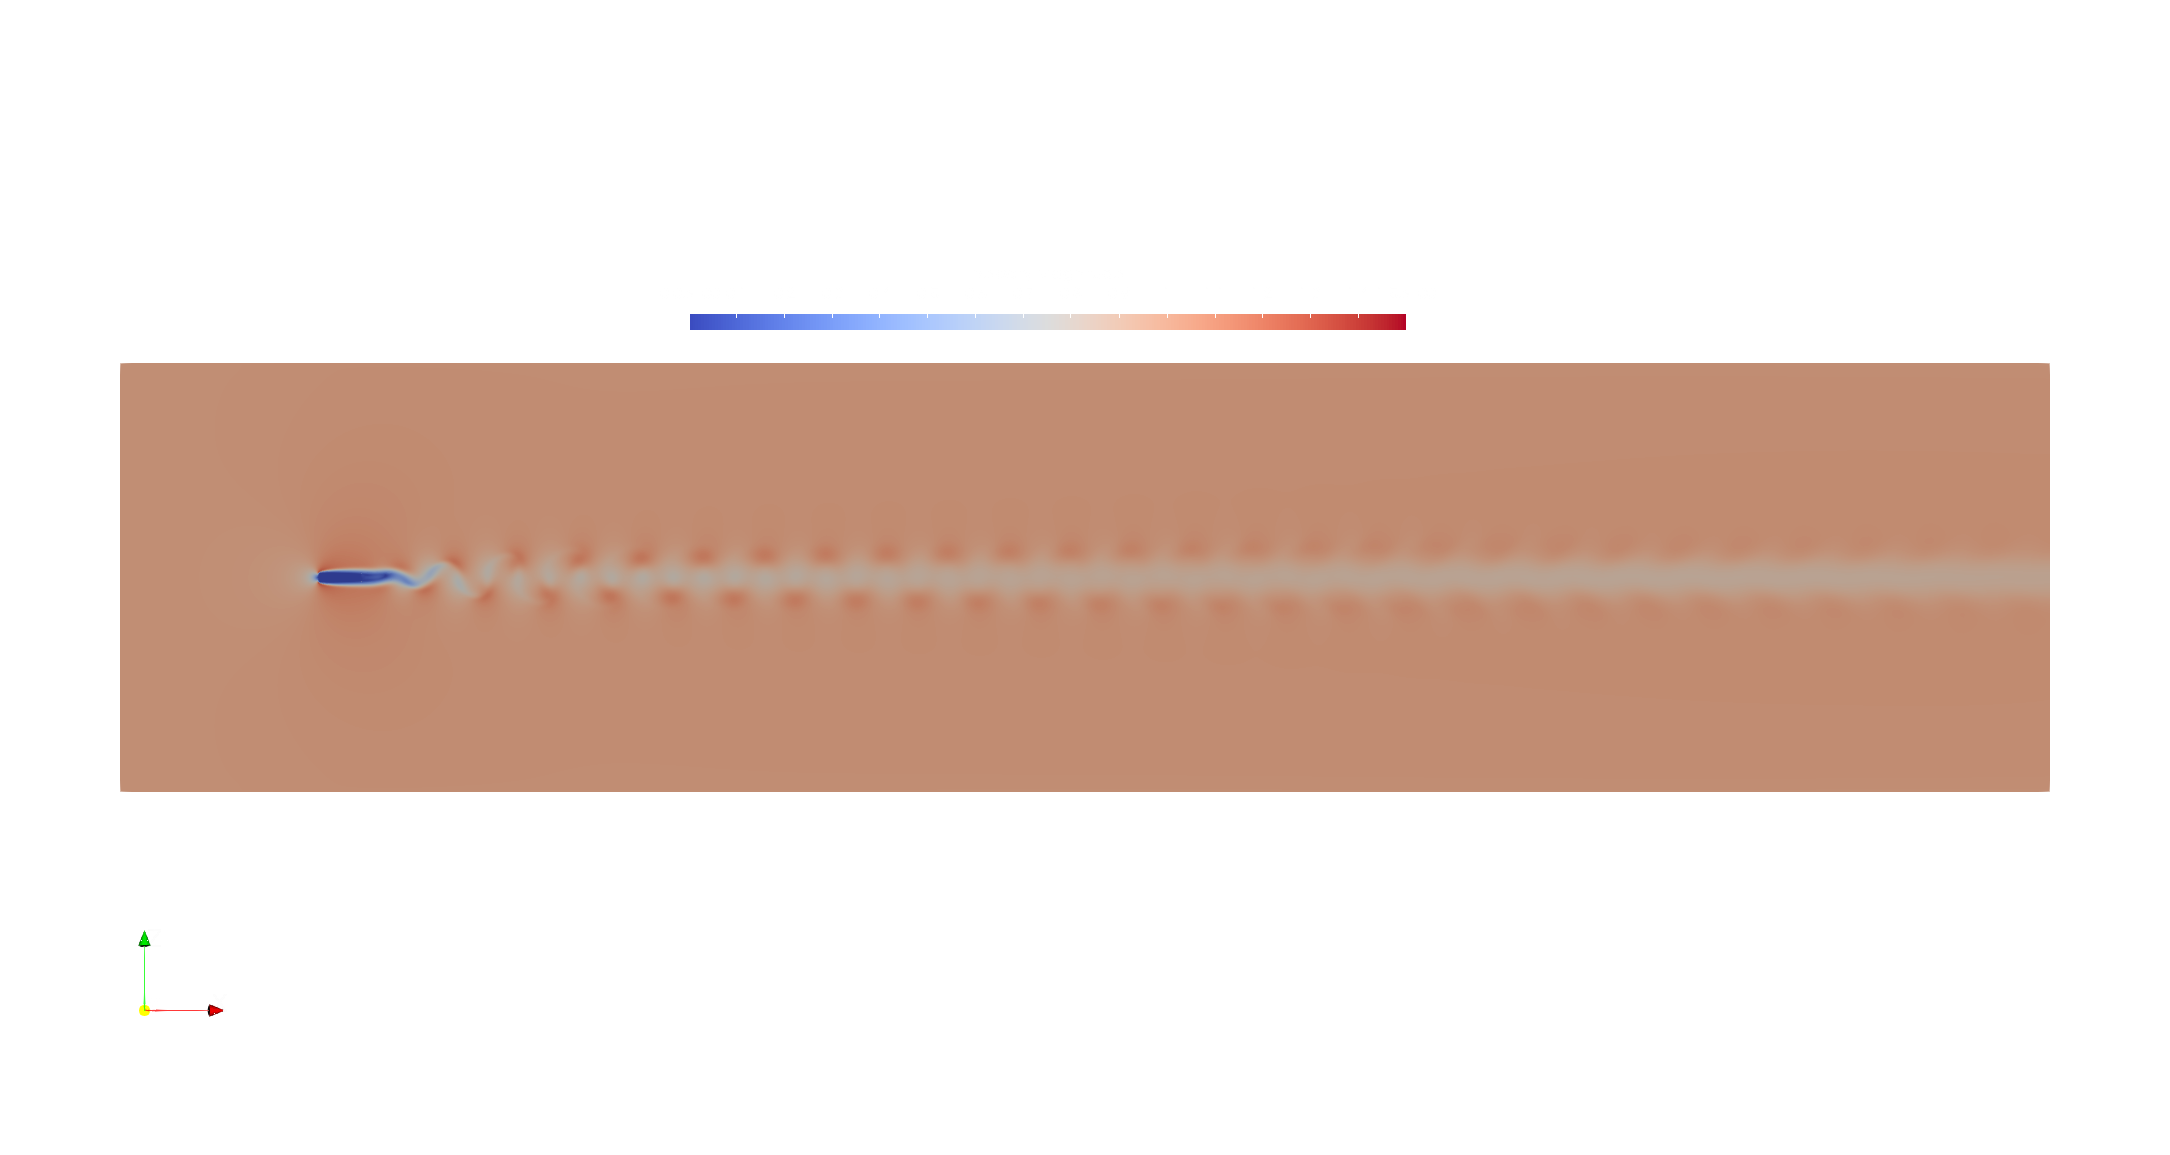
\includegraphics[trim={0 9cm 0 13cm},clip,width=0.5\textwidth]{AR5Re150.png}};
  \node (origin) at (0.3,0)   { $Re=150$};    
  
   \node (origin) at (6,-1)   { 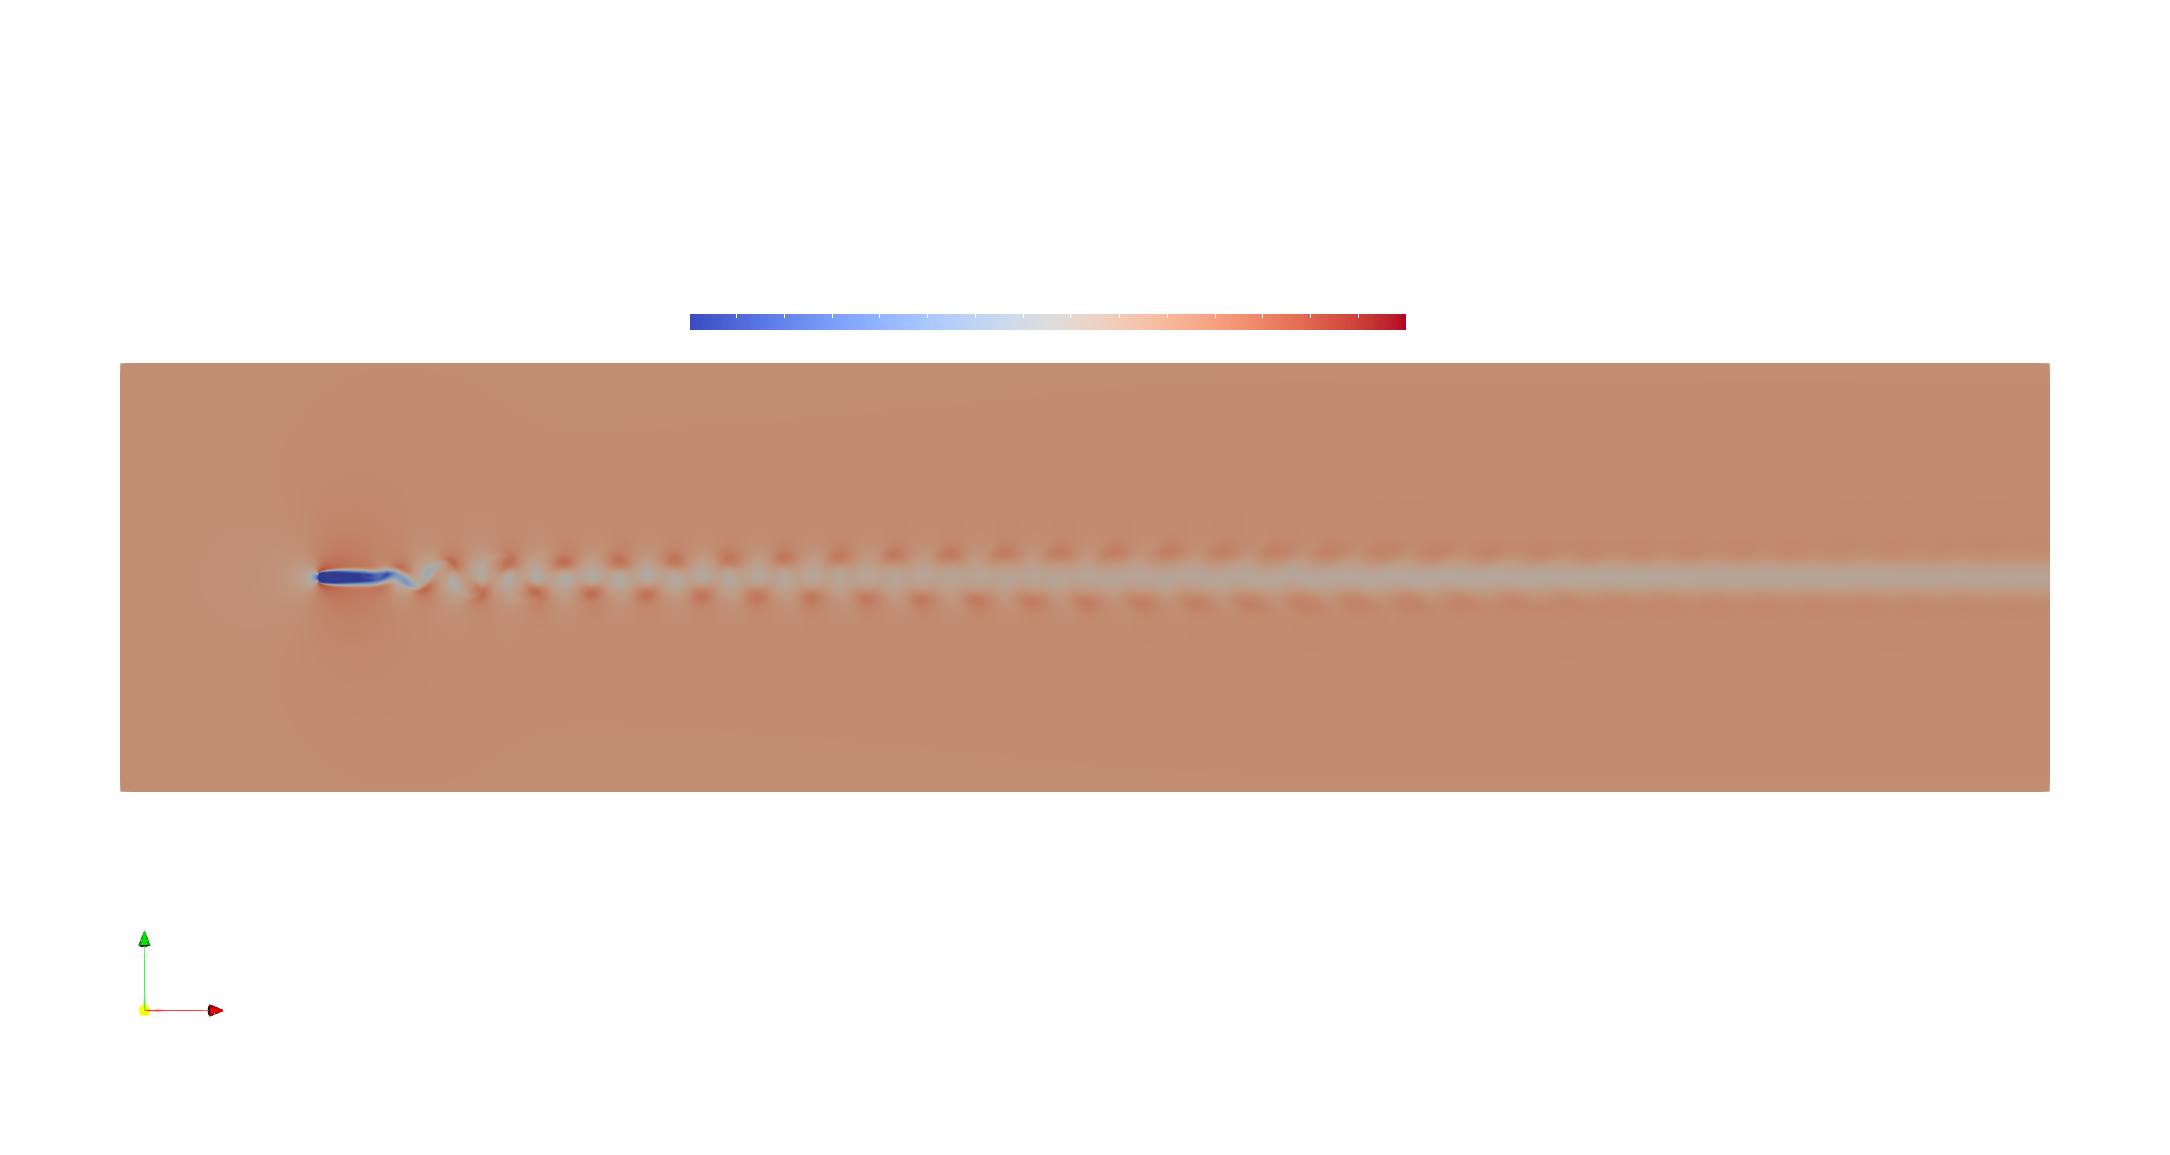
\includegraphics[trim={0 9cm 0 13cm},clip,width=0.5\textwidth]{AR5Re200.png}};
  \node (origin) at (6.45,0)   { $Re=200$};  
  
  \node (origin) at (-0.15,-3)   { 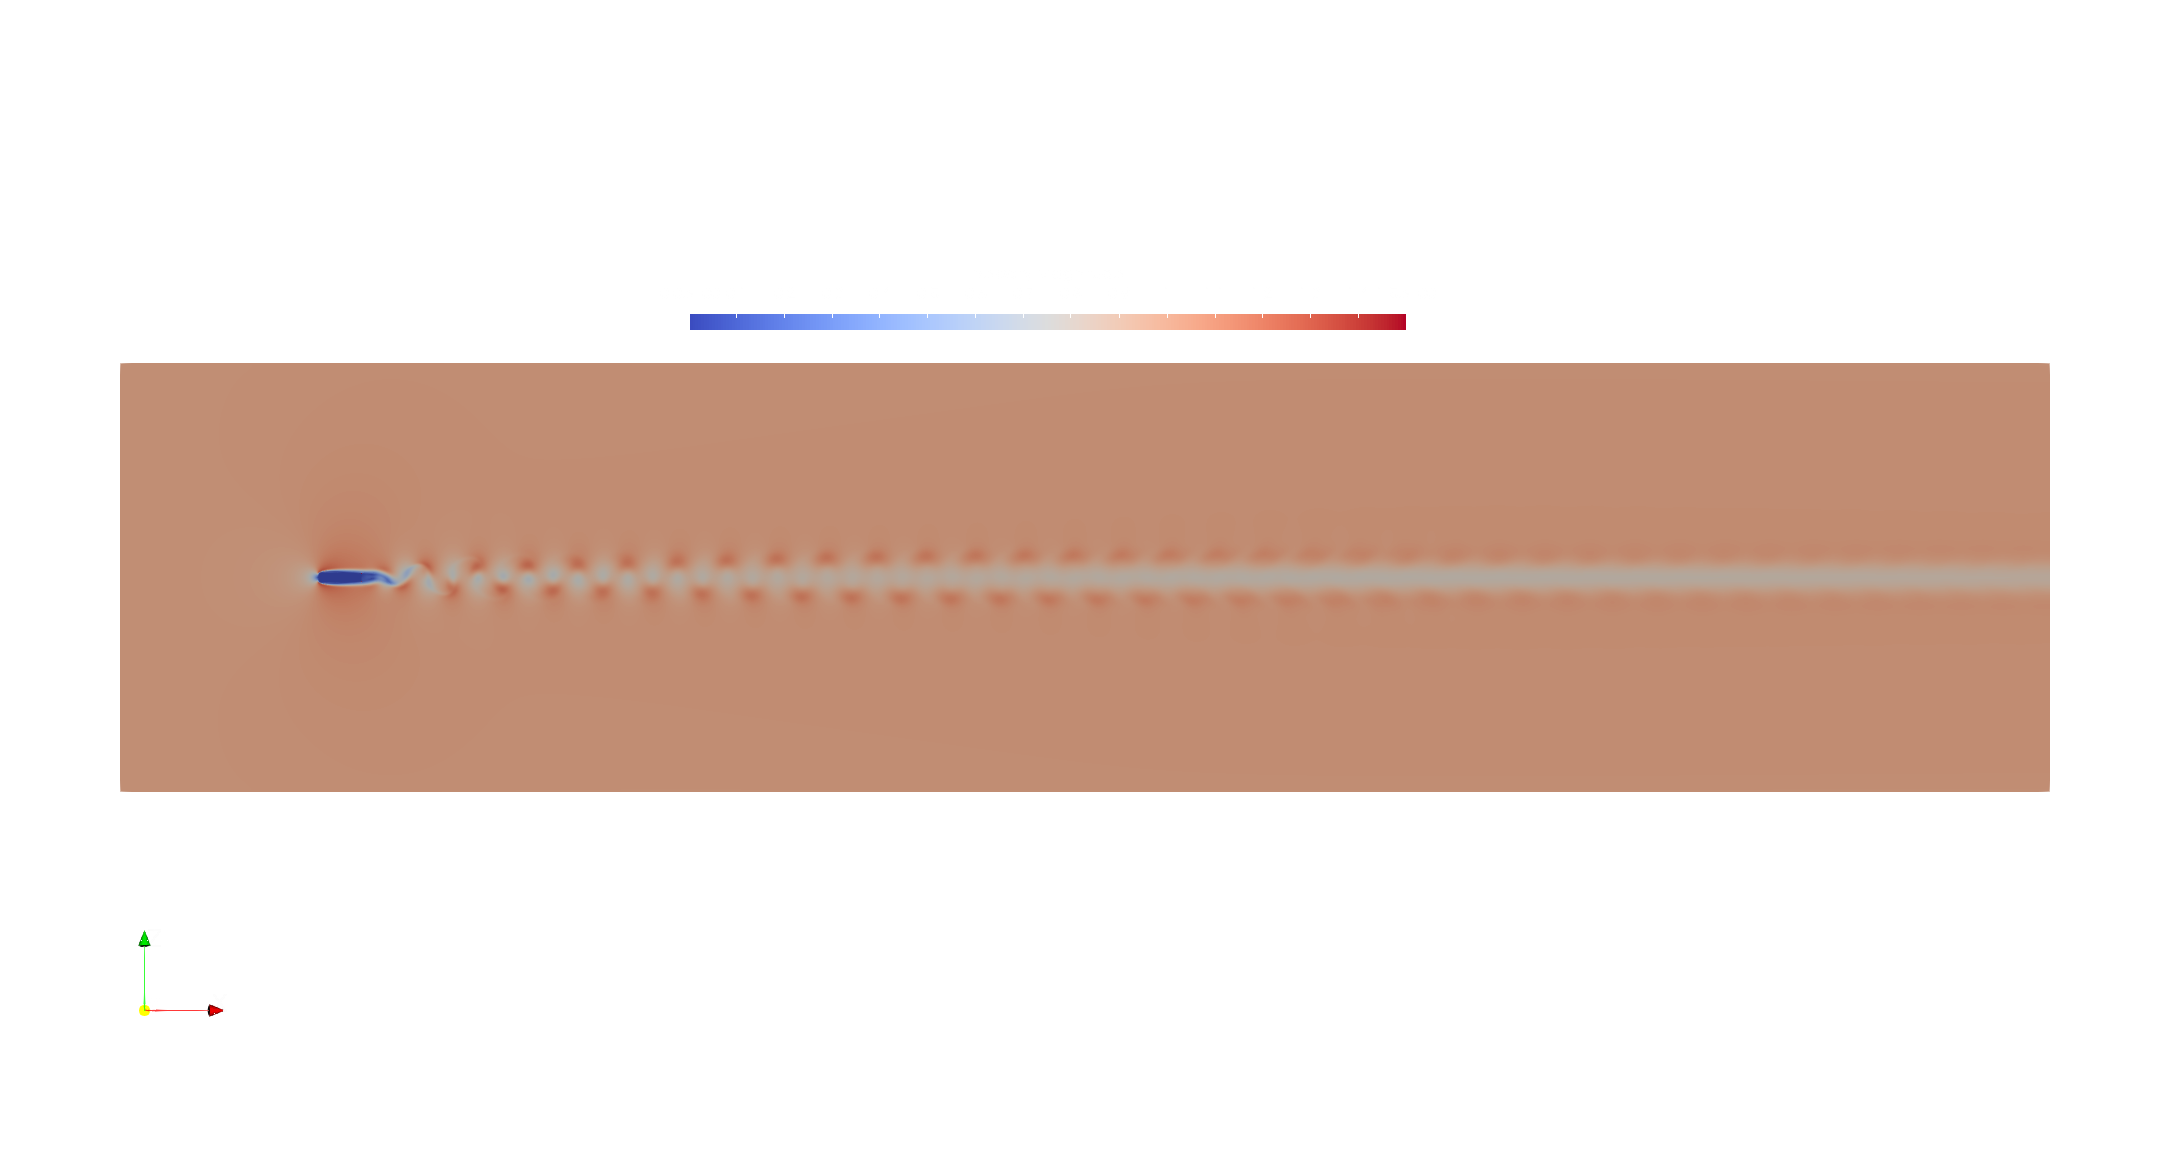
\includegraphics[trim={0 9cm 0 13cm},clip,width=0.5\textwidth]{AR5Re250.png}};
  \node (origin) at (0.3,-2)   { $Re=250$};    
  
   \node (origin) at (6,-3)   { 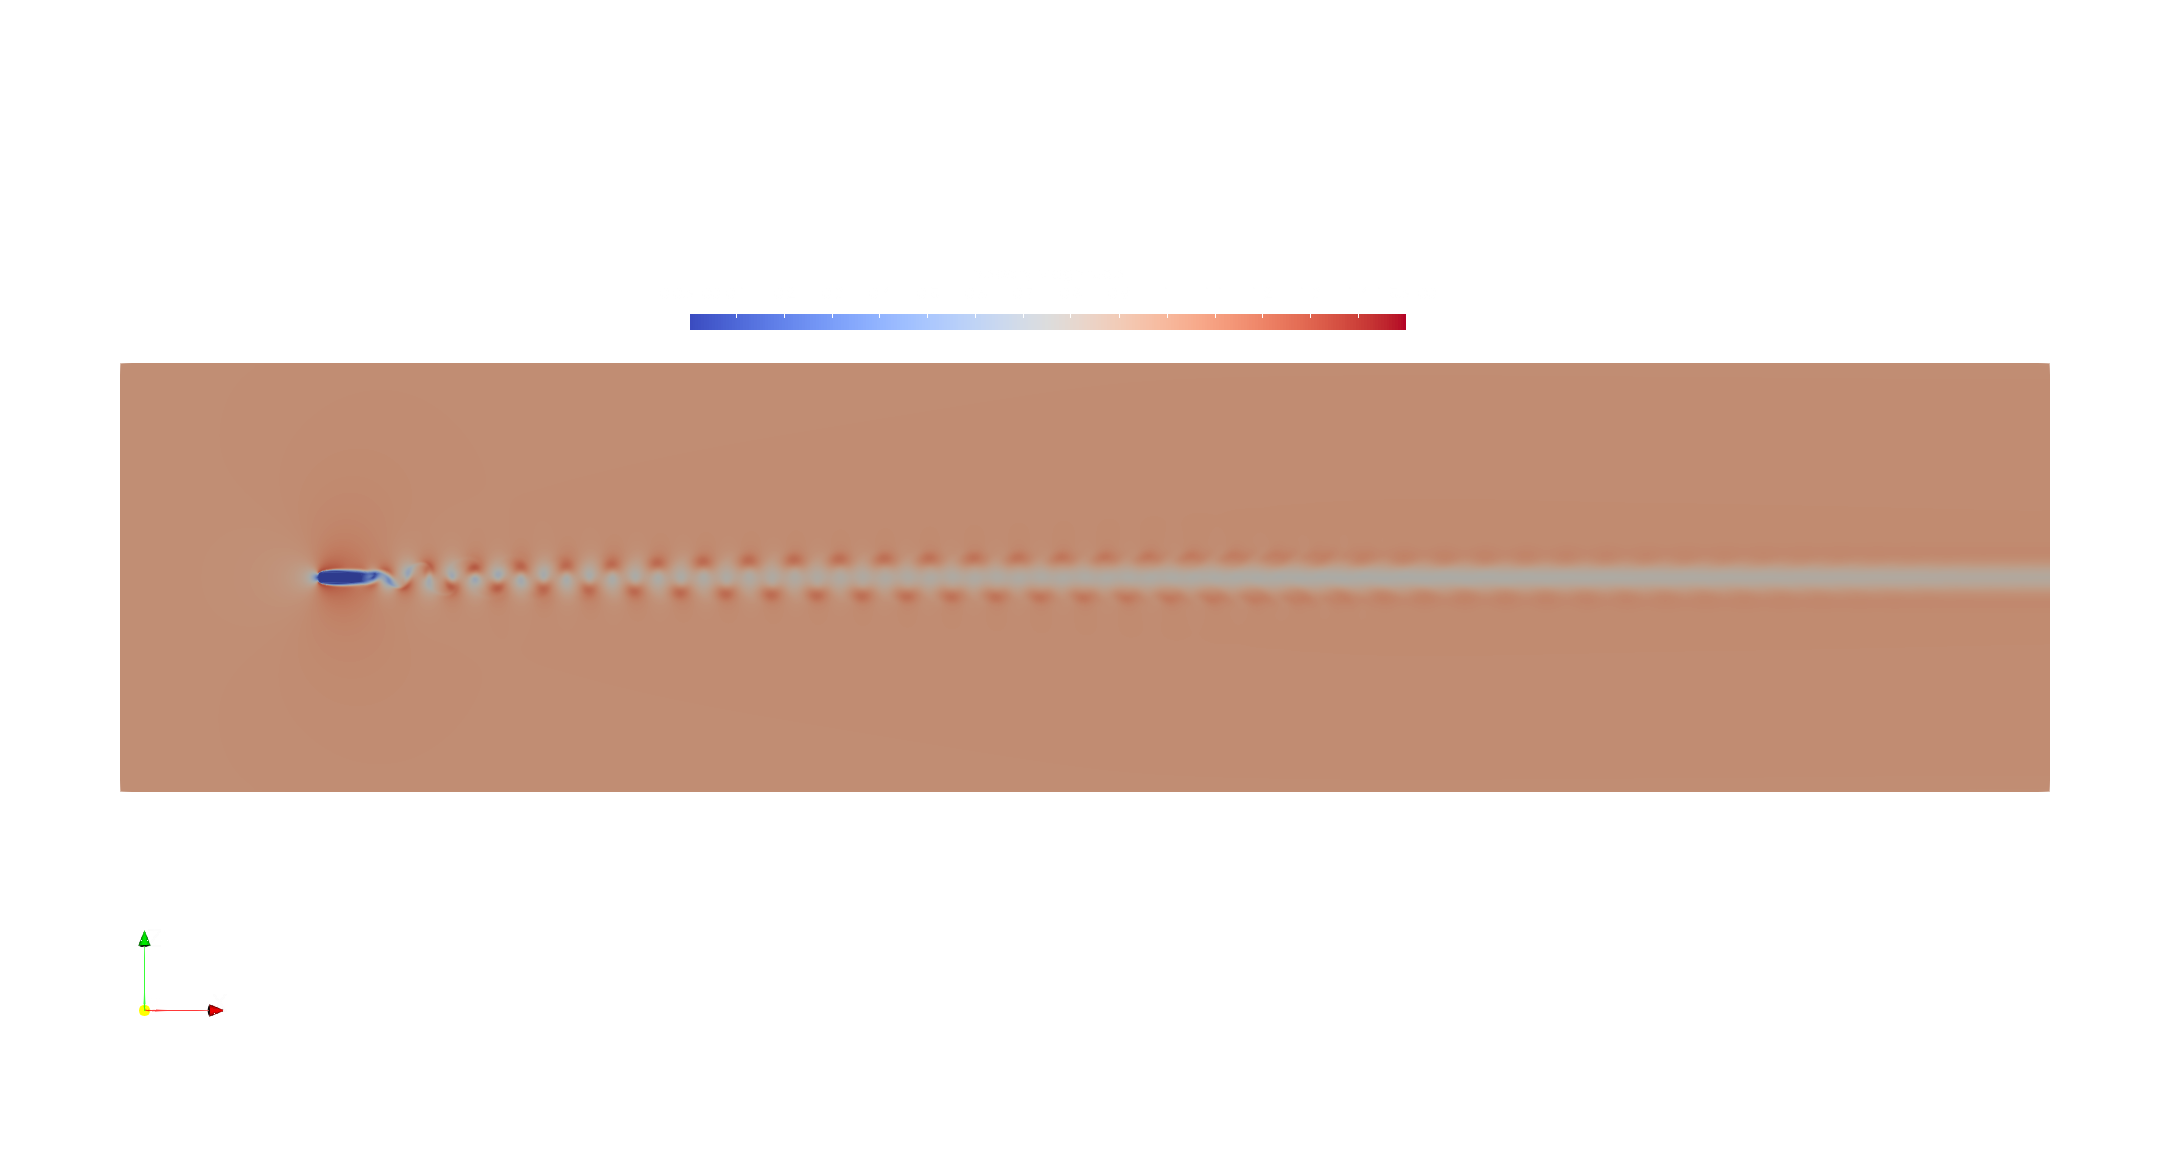
\includegraphics[trim={0 9cm 0 13cm},clip,width=0.5\textwidth]{AR5Re300.png}};
  \node (origin) at (6.45,-2)   { $Re=300$};    
  
  \node (origin) at (-0.15,-5)   { 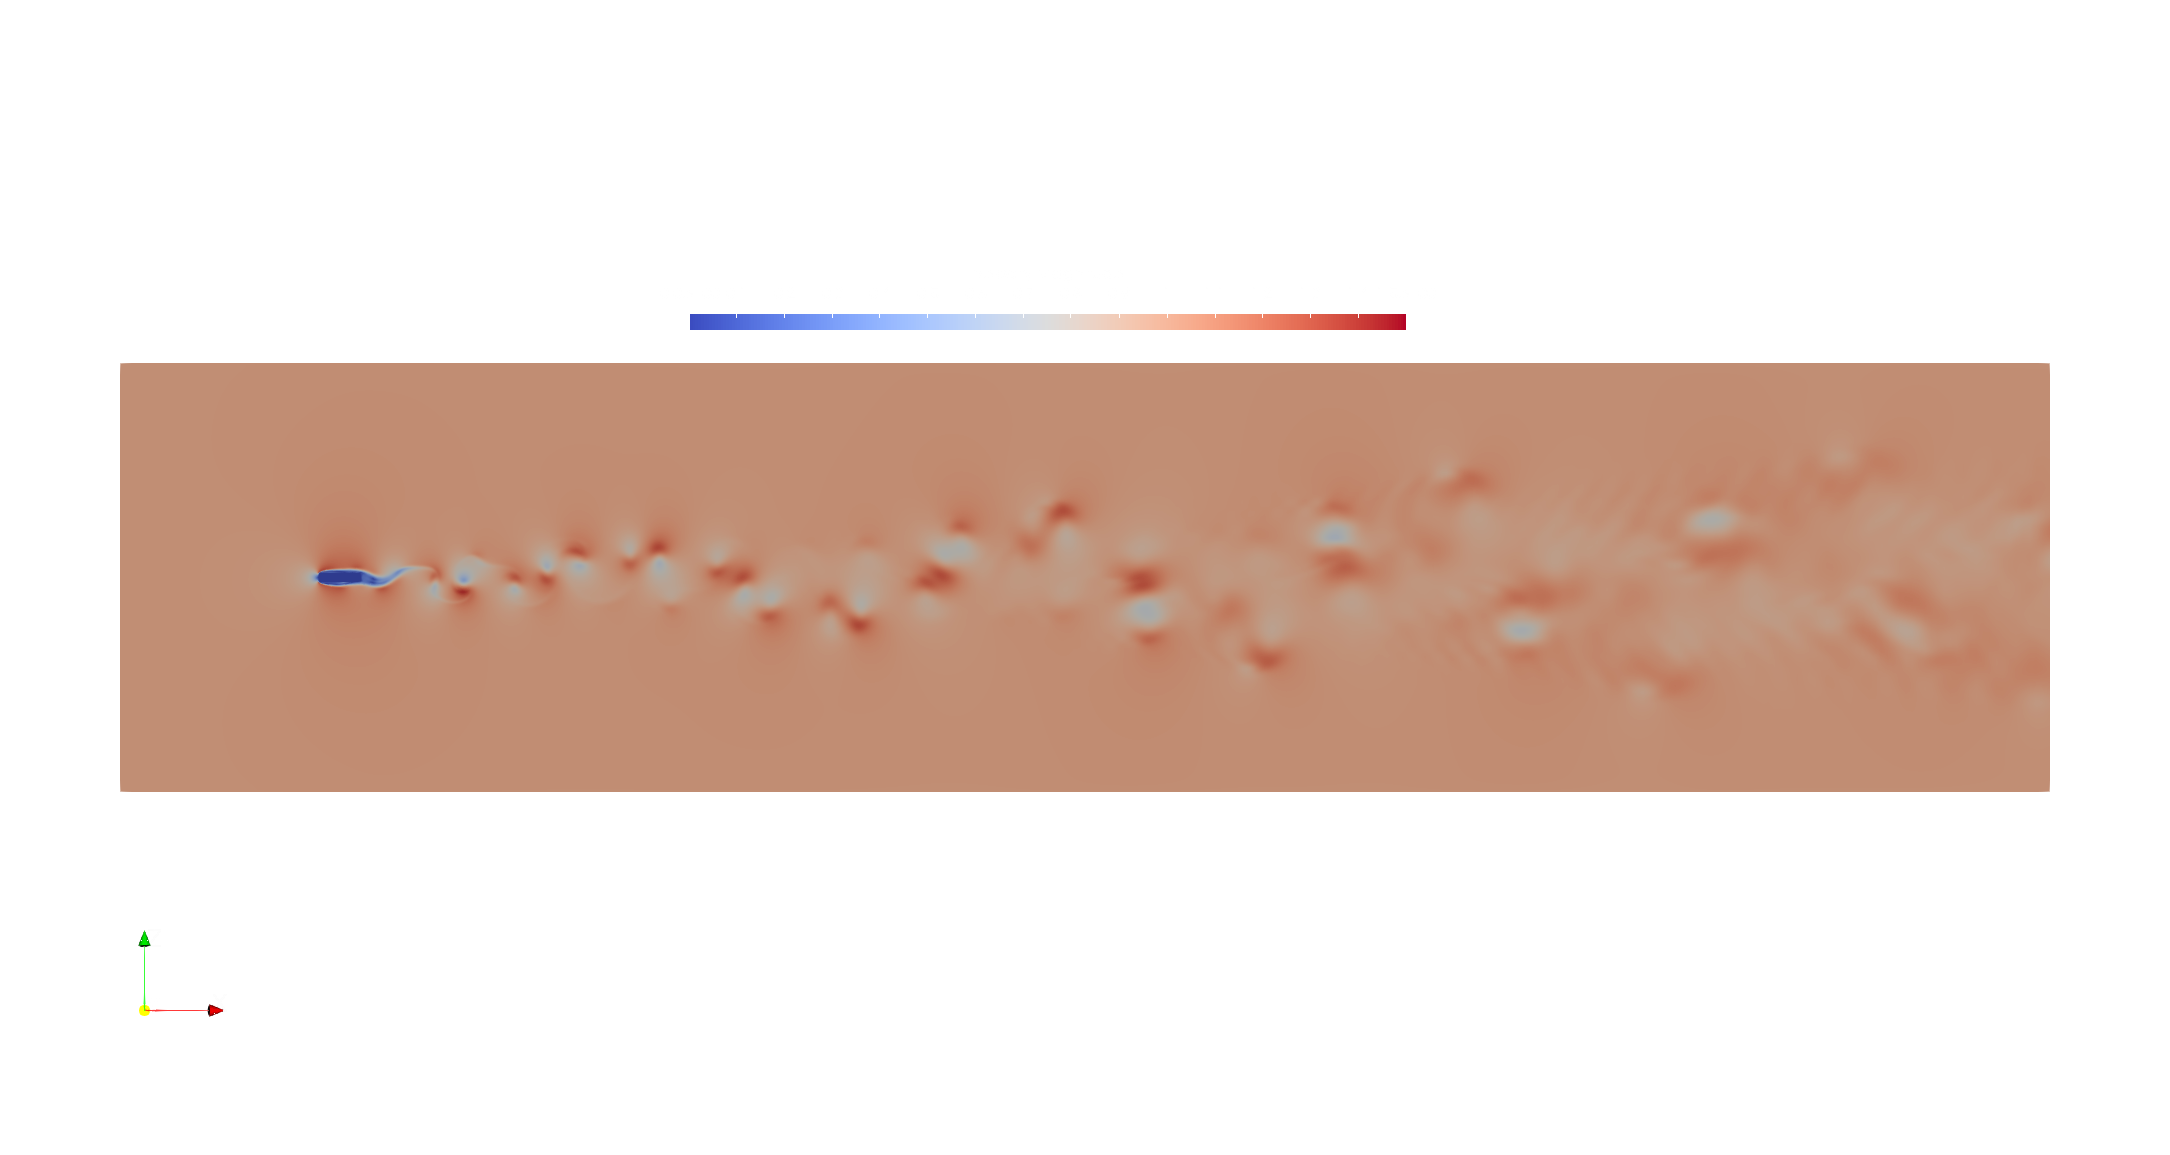
\includegraphics[trim={0 9cm 0 13cm},clip,width=0.5\textwidth]{AR5Re350.png}};
  \node (origin) at (0.3,-4)   { $Re=350$};    
  
   \node (origin) at (6,-5)   { 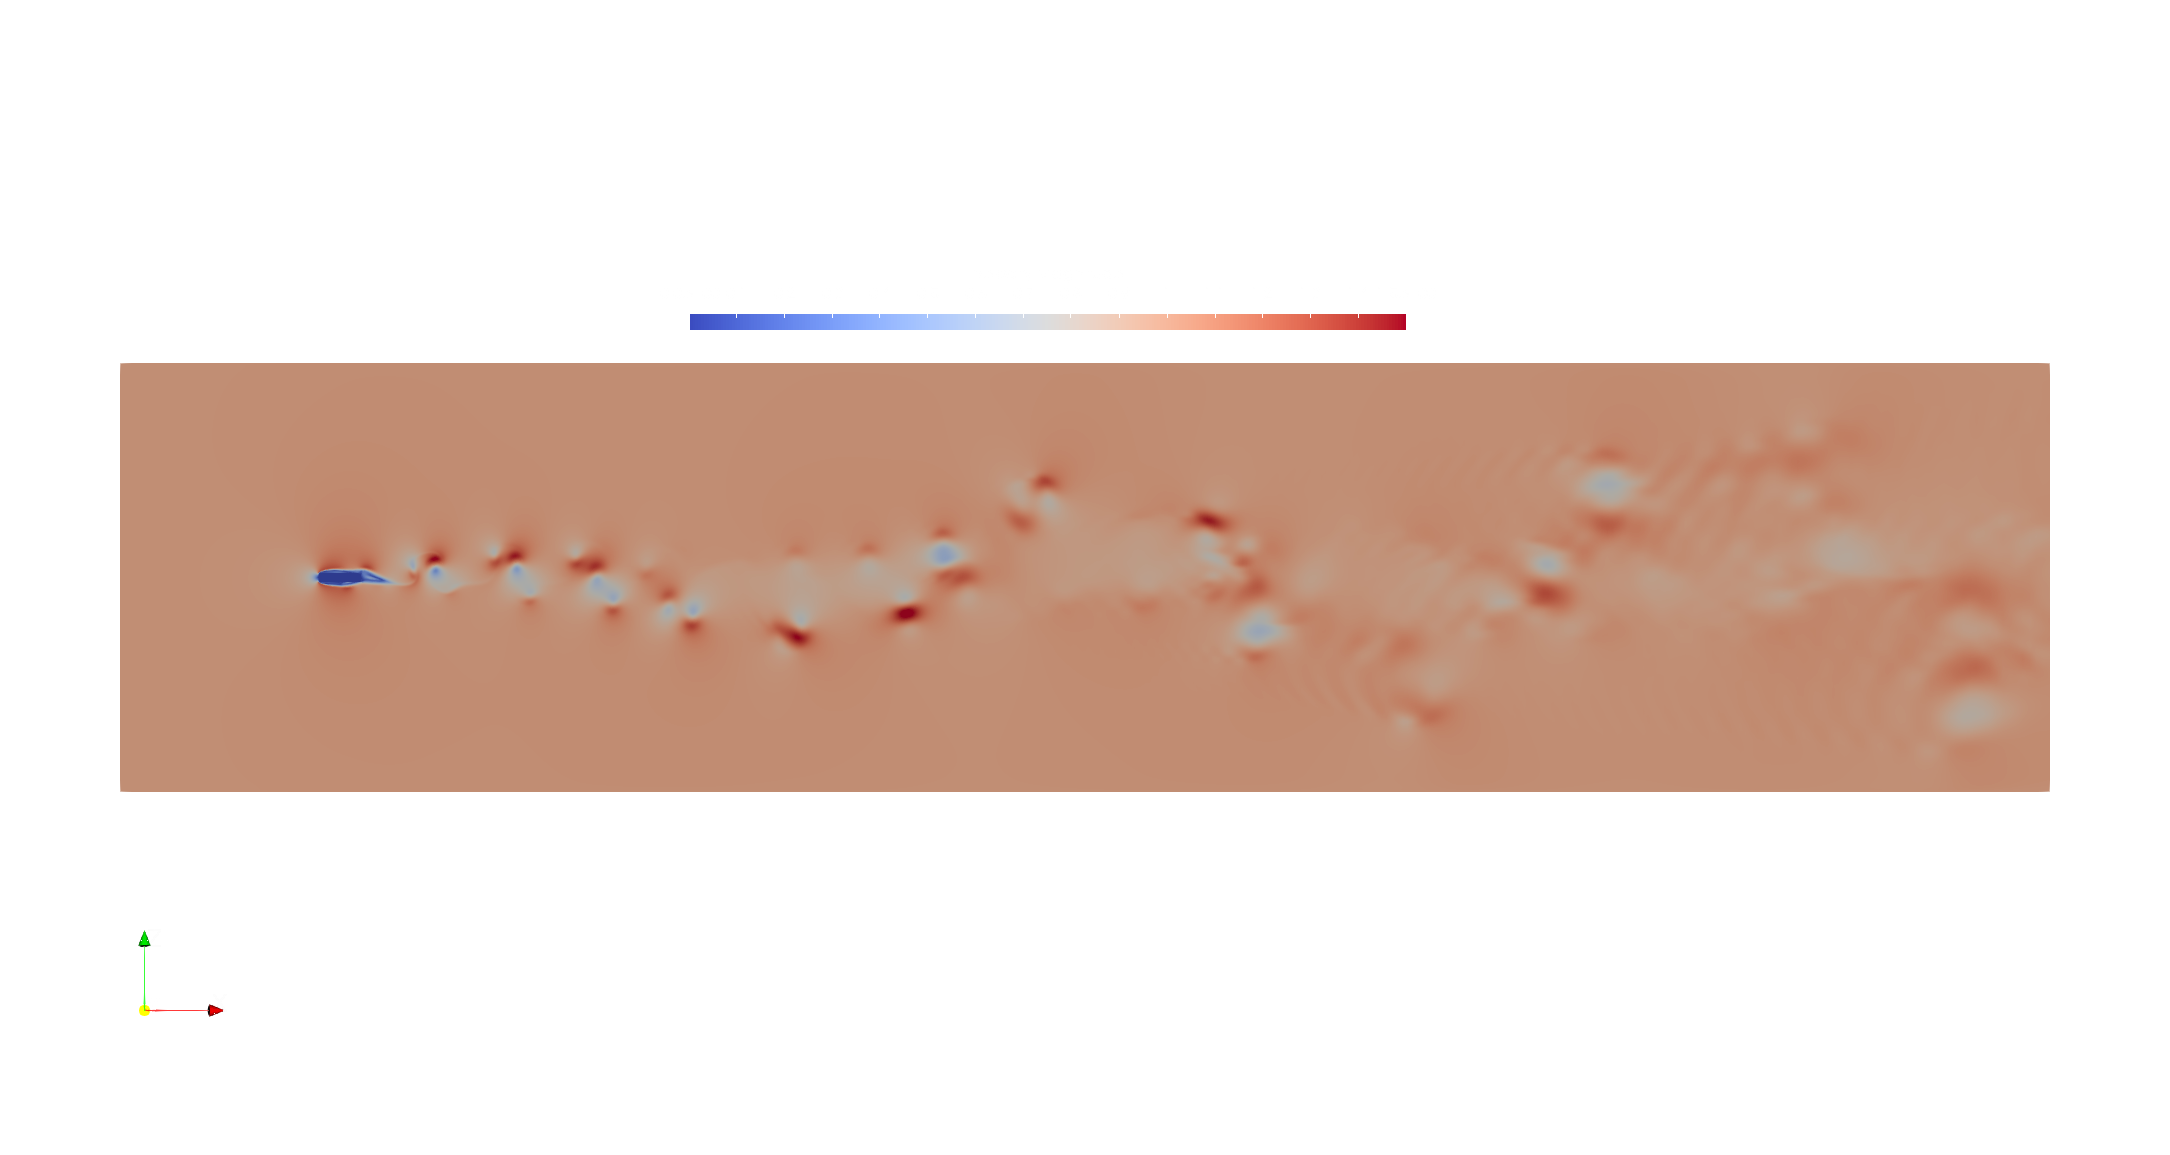
\includegraphics[trim={0 9cm 0 13cm},clip,width=0.5\textwidth]{AR5Re400.png}};
  \node (origin) at (6.45,-4)   { $Re=400$};            
            

\end{tikzpicture}
\end{document}
